\documentclass[svgnames, 12pt]{beamer}

\usepackage[utf8]{inputenc}
\usepackage[english]{babel}
\usepackage[L7x]{fontenc}
\usepackage{amsmath}
\usepackage{amssymb}
\usepackage{lmodern}
\usepackage{xcolor}
\usepackage{subfig}
\usepackage{graphicx}
\usepackage{listings}

\definecolor{mifcolor}{RGB}{0, 71, 127}
\definecolor{dimgr}{RGB}{105, 105, 105}
\definecolor{sky}{RGB}{0, 191, 255}
\setbeamercolor{alerted text}{fg=red,bg=sky}

\definecolor{codegreen}{rgb}{0,0.6,0}
\definecolor{codegray}{rgb}{0.5,0.5,0.5}
\definecolor{codepurple}{rgb}{0.58,0,0.82}
\definecolor{backcolour}{rgb}{0.95,0.95,0.92}

\lstdefinestyle{mystyle}{
    backgroundcolor=\color{backcolour},   
    commentstyle=\color{codegreen},
    keywordstyle=\color{magenta},
    numberstyle=\tiny\color{codegray},
    stringstyle=\color{codepurple},
    basicstyle=\ttfamily\small,
    breakatwhitespace=false,         
    breaklines=true,                 
    captionpos=b,                    
    keepspaces=true,                 
    numbers=left,                    
    numbersep=5pt,                  
    showspaces=false,                
    showstringspaces=false,
    showtabs=false,                  
    tabsize=2
}

\lstset{style=mystyle}

\mode<presentation>{
\usetheme{Madrid}
\usecolortheme[named=mifcolor]{structure}
}

\title{Big Data Analysis - Assignment 1}
\author{Davide Griffon}
\institute{Vilnius University}
\date{\today}

\begin{document}

% Slide 1 - Title
\begin{frame}
\titlepage
\end{frame}

% Slide 2 - Overview
\begin{frame}{Project Overview}
    \begin{columns}[T] % T for top alignment
    \column{0.5\textwidth}
    \textbf{Anomaly Types:}
    \begin{itemize}
        \item \textbf{Vessel movement anomalies}
        \begin{itemize}
            \item Speed inconsistencies
            \item AIS transmission time gaps
        \end{itemize}
        \item \textbf{Location anomalies}
        \begin{itemize}
            \item Position conflicts between vessels
        \end{itemize}
    \end{itemize}
    
    \column{0.5\textwidth}
    \textbf{Technical Approach:}
    \begin{itemize}
        \item Spatiotemporal binning for efficient processing
        \item Parallel computing with multiprocessing
        \item Vectorized operations (pandas/numpy)
        \item Unit testing with pytest
        \item Structured development with Taskfile
    \end{itemize}
    \end{columns}
\end{frame}

% Slide 3 - Vessel Movement Anomalies
\begin{frame}{Vessel Movement Anomaly Detection}
    \begin{itemize}
        \item \textbf{Two primary indicators:}
        \begin{itemize}
            \item \textbf{Speed anomalies}: Vessels reporting unrealistic speeds
            \item \textbf{AIS gaps}: Unusually long periods between transmissions
        \end{itemize}
        \item \textbf{Implementation approach:}
        \begin{itemize}
            \item Group data by vessel MMSI
            \item Calculate distances between consecutive points using geopy
            \item Vectorized operations for time differences and speed calculations
            \item Flag vessels exceeding a threshold (default 50.0 miles/h)
            \item Flag transmission gaps exceeding a threshold (default 1.0 hour)
        \end{itemize}
        \item \textbf{Optimization:}
        \begin{itemize}
            \item Process each vessel independently (perfect for parallelization)
            \item Use of NumPy for vectorized distance calculations
        \end{itemize}
    \end{itemize}
\end{frame}

% Slide 4 - Location Anomalies (Part 1)
\begin{frame}{Location Anomaly Detection - Binning}
    \begin{columns}
    \column{0.6\textwidth}
    \textbf{Spatiotemporal Binning:}
    \begin{itemize}
        \item Challenge: Efficiently finding vessels at same location/time
        \item Solution: Group data into spatial and temporal bins
        \begin{itemize}
            \item latitude "edge" = 0.01° (\textasciitilde1km)
            \item longitude "edge" = 0.01° (varies)
            \item temporal bin = "1min"
        \end{itemize}
        \item Boundary handling:
        \begin{itemize}
            \item Points near bin boundaries are placed in multiple bins
            \item Prevents missing conflicts at bin edges
        \end{itemize}
    \end{itemize}
    
    \column{0.4\textwidth}
    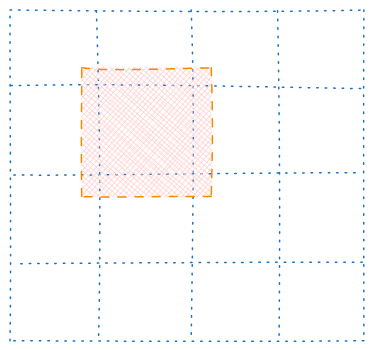
\includegraphics[width=\textwidth]{images/spatial_binning.png}
    {\tiny \textit{Illustration of spatial binning with overlap}}
    \end{columns}
\end{frame}

% Slide 5 - Location Anomalies (Part 2)
\begin{frame}{Location Anomaly Detection - Finding Conflicts}
    \textbf{Conflict Detection Process:}
    \begin{enumerate}
        \item Preprocess data
        \begin{itemize}
            \item Apply spatial binning
            \item Apply temporal binning
            \item Group by lat/lon/time bins
        \end{itemize}
        \item Process each chunk/bin in parallel
        \begin{itemize}
            \item Create position-time hash for efficient lookup
            \item Find exact position and time matches
            \item Identify vessels with different MMSIs at identical positions
        \end{itemize}
        \item Combine results and remove duplicates
        \begin{itemize}
            \item Keep only one conflict per vessel pair (smallest distance)
            \item Sort by distance for easier analysis
        \end{itemize}
    \end{enumerate}
\end{frame}

% Slide 6 - Results 
\begin{frame}{Performance Results} 
    \begin{columns}[t]
      \column{0.5\textwidth} 
      \textbf{Dataset Characteristics:} 
      \begin{itemize} 
        \item 5,901 unique vessels (MMSI) analyzed 
        \item 36,583 spatiotemporal bins processed 
        \item Full day of AIS data (aisdk-2024-06-30.csv) 
      \end{itemize} 
      
      \column{0.5\textwidth} 
      \textbf{Performance Comparison:} 
      \begin{itemize} 
        \item \textbf{Single-process:} 780 seconds 
        \item \textbf{Multi-process:} 230 seconds 
        \item \textbf{Speedup:} 3.4x 
      \end{itemize} 
    \end{columns} 
    
    \vspace{0.5cm} 
    \textbf{Conclusion:} Parallel processing provides significant performance improvement for spatiotemporal anomaly detection in vessel tracking data. 
    \end{frame}

\end{document}